\documentclass{article}

\textwidth=6.5in
\textheight=8.5in
\voffset=-54pt
\oddsidemargin=0in
\evensidemargin=0in
\setlength{\parskip}{8pt}
\setlength{\parindent}{0pt}

\usepackage{workbook}

\usepackage[]{handout}
\renewcommand{\workshopnote}{CA Notes.} 
\usepackage{lipsum}
 \usepackage{microtype}
 \usepackage{vwcol}
\begin{document}

\htitle{Workshop 4: Derivatives of Trig Functions and their Applications}

\begin{workshop}
    The goals of this workshop are for students to
    \begin{itemize}
        \item recall the derivatives of $\sin x$ and $\cos x$, and use them to derive the derivatives of $\tan x$, $\cot x$, $\csc x$, and $\sec x$.
        \item compute derivatives of trig functions using a variety of derivative rules (Product Rule, Chain Rule) and techniques (implicit differentiation, logarithmic differentiation). 
        \item solve related rates problems involving trigonometric functions.
    \end{itemize}
    
    If time permits, students can also
    \begin{itemize}
    \item practice curve sketching with oscillating functions.
    \item explore the utility of envelope functions while sketching oscillating functions.
    \end{itemize}
Students should be able to complete \#1 and \#2 independently, so these might be good problems for table work. On the other hand, \#3 and \#4 are much more computationally heavy, so students can elect to work in groups at the boards on these problems (for collaboration and clarity purposes). \#5 is likely going to be a challenging related rates problem for most students, so please have students collaborate on \#5 at the boards, and leave at least 30 to 40 minutes to work on this problem, including time to debrief. You will likely not have time to work on \#6 and \#7, which is fine because some of it is exploratory material.
\end{workshop}

 \begin{framed}
    \textbf{Derivatives of the six basic trigonometric functions.}  (You
    should memorize these.)

    \begin{multicols}{3}
    
      $\dfrac{d}{dx} (\sin x) = \fitb{1in}{
      \solonly\textcolor{red}{\cos x}
      }$

      $\dfrac{d}{dx} (\csc x) = - \csc x \cot x$

      $\dfrac{d}{dx} (\cos x) = \fitb{1in}{\solonly\textcolor{red}{-\sin x}}$

      $\dfrac{d}{dx} (\sec x) = \sec x \tan x$

      $\dfrac{d}{dx} (\tan x) = \fitb{1in}{\solonly\textcolor{red}{\sec ^2 x}}$

      $\dfrac{d}{dx} (\cot x) = -\csc^2 x$
      
    \end{multicols}
    
  \end{framed}
  \begin{enumerate}
\item Suppose you can't remember $\frac{d}{dx} \sec x$. First express $\sec x$ in terms of $\sin x$ or $\cos x$, then differentiate with respect to $x$. (Note: You can do this with $\tan x$, $\cot x$, and $\csc x$ as well.)

\begin{solution}
Recall that $\sec x = \dfrac{1}{\cos x}$, which can be rewritten as $\sec x =(\cos x)^{-1}$. Differentiating starting with Chain Rule,
\begin{align*}
\frac{d}{dx}\left[(\cos x)^{-1}\right]&=-(\cos x)^{-2}\cdot(-\sin x)\\
&=\frac{\sin x}{(\cos x)^{2}}\\
&=\frac{1}{\cos x} \cdot \frac{\sin x}{\cos x}\\
&=\sec x \tan x
\end{align*}
\end{solution}
\vfill\vfill
  \item Compute the derivatives of the following functions.
  \begin{enumerate}

    \item $f(x)=\sin(x^2-1)$
    
    \begin{solution}
        $f'(x)=\cos(x^2-1)\cdot2x$
    \end{solution}
    
    \vfill
    
    \item $g(x)=\ln (\cos x)$
    
    \begin{solution}
        $g'(x)=\dfrac{1}{\cos x}\cdot(-\sin x)=-\tan x$
    \end{solution}
    
    \vfill
    \item $h(x)=\tan^3 x$ 
    
    \begin{solution}
        $h'(x)=3\tan^2 x\cdot \sec ^2 x$
    \end{solution}
    \vfill
    \item $k(x)= \sec(x^2)$
    
    \begin{solution}
        $k'(x)=\sec(x^2)\tan(x^2)\cdot2x$
    \end{solution}
    \vfill

    \end{enumerate}
\newpage
\begin{workshop}
    This is an exam-type problem. If you choose to bring the class together to debrief this problem, please be sure to use parentheses and brackets as needed and highlight our need for them if terms with a lot of groupings begin to pile up. Students tend to get caught up in memorizing steps for logarithmic differentiation; please display your board work logically and provide reasons for the steps you take in your process.
\end{workshop}
\item Find $m'(x)$ if $m(x)=x^{\cos x}$. 

\begin{solution}
    Because $m(x)$ is a function that takes the form of $f(x)^{g(x)}$, let's use logarithmic differentiation to find $m'(x)$:
    \begin{align*}
        \ln[m(x)]&=\ln(x^{\cos x}) \\
        \ln[m(x)]&=\cos x\cdot\ln x \\
        \frac{d}{dx}\Biggl[\ln[m(x)]\Biggr]&=\frac{d}{dx}(\cos x\cdot\ln x) \\
        \frac{1}{m(x)}\cdot m'(x)&= -\sin x \cdot \ln x + \cos x \cdot \frac{1}{x} \\
        \frac{m'(x)}{m(x)}&= -\sin x \cdot \ln x + \frac{\cos x}{x} \\ 
        m'(x)&= m(x)\left[-\sin x \cdot \ln x + \frac{\cos x}{x}\right] \\ 
         m'(x)&=x^{\cos x}\left[-\sin x \cdot \ln x + \frac{\cos x}{x}\right]
    \end{align*}
\end{solution}
\vfill\vfill

\begin{workshop}
    This is an exam-type problem. If you choose to bring the class together to debrief this problem, please be sure to highlight moments when implicit differentiation is required, and how to handle these moments when product rule or sum rule for derivatives is needed in tandem. Please avoid explicitly solving for $\frac{dy}{dx}$ before plugging in $x=2$ and $y=0$, as this generates an unnecessary amount of computation prone to algebraic errors.
\end{workshop}

\item Find the slope of the line tangent to the curve $\sin(\pi x+y) = \cos(xy) - 1$ at $(2, 0)$. (Recall that you need not explicitly solve for $\dfrac{dy}{dx}$ after differentiating in order to answer this question). 

\begin{solution}
\begin{align*}
    \frac{d}{dx} \biggl[\sin(\pi x+y)\biggr] &= \frac{d}{dx}\biggl[\cos(xy) - 1\biggr] \\
    \cos(\pi x+y)\cdot\left(\pi + \frac{dy}{dx}\right) &= -\sin(xy)\cdot \left(y+x\cdot\frac{dy}{dx}\right) \\
    \cos(2\pi+0)\cdot\left(\pi + \frac{dy}{dx}\right) &= -\sin(2\cdot0)\cdot \left(0+2\cdot\frac{dy}{dx}\right) \\
     1\cdot\left(\pi + \frac{dy}{dx}\right) &= 0\cdot \left(2\cdot\frac{dy}{dx}\right) \\
       \pi + \frac{dy}{dx} &= 0 \\
      \frac{dy}{dx} &= -\pi \\
\end{align*}
\end{solution}
\vfill\vfill\vfill

\newpage
\begin{workshop}
    This is an exam-type problem, albeit a bit long and scaffolded.
\end{workshop}
\item In this question you will work on the following related rates problem:

    

\textit{A hungry lion is running down a straight jungle path at a rate of $60$ feet per second.  A meerkat is hiding in a bush $20$ feet away perpendicular to the
jungle path, hoping that the lion will not eat him.  As the lion runs, the meerkat turns his head so as to keep an eye on the lion.  At the moment when the lion is $40$ feet from the meerkat and getting closer,}

    \begin{itemize}
    \item \textit{how fast is the meerkat's head turning (in radians per second)?}
    \item \textit{at what rate is the distance between the lion and the meerkat shrinking?}
    \end{itemize}
\begin{enumerate}
\item 
\begin{workshop}
    Students may have a hard time describing what some variables represent without a picture in place, so it might be helpful to look at part (a) and part (b) at the same time.
\end{workshop}

    Define and assign variables to the three quantities that change with respect to time in this scenario.
    \begin{itemize}
        \item \solonly{the distance $z$ between the lion and the meerkat}\phantom{text}
        \probonly{\newline}
        \item \solonly{the angle $\theta$ between the meerkat's line of sight and the jungle path 20 feet away} \phantom{text}
      \probonly{\newline}
        \item \solonly{the lion's position $y$ (with respect to the jungle path 20 feet away from the meerkat)}\phantom{text}
       \probonly{\newline}
    \end{itemize}
    \item 
    \begin{workshop}
        Nonetheless, it is essential that students include variables in their generic picture that vary with respect to time in the given scenario. The only ``constant" in this scenario that is ``always true" is the $20$ foot distance between the path and the bush, so this is the only constant that should appear in the generic picture.
    \end{workshop}
    Using the variables named above, draw and label a general picture that models the scenario. 
    
    \begin{solution}
    \begin{center}
        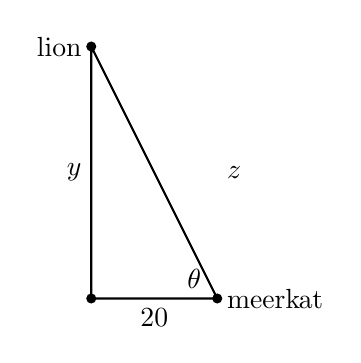
\begin{tikzpicture}[scale=0.4]
     \draw[thick](0,0) -- (0,-8) -- (4,-8) -- (0,0);
     \node[left] at (0,0){lion};
     \node[left] at (0,-8){};
     \node[right] at (4,-8){meerkat};
      \node[anchor=south east] at (3.8,-8){$\theta$};
     \draw[fill] (0,0) circle [radius=4pt];
     \draw[fill] (0,-8) circle [radius=4pt];
     \draw[fill] (4,-8) circle [radius=4pt];
     \node[left] at (0,-4){$y$};
     \node[below] at (2,-8){$20$};
     \node[right] at (4,-4){$z$};
    
     \end{tikzpicture}
     \end{center}
    \end{solution}
    \vfill\vfill
    \item Using the variables named above and derivative notation, identify the two goals of the problem.
    
    \begin{solution}
        $\frac{d\theta}{dt}$ and $\frac{dz}{dt}$ when $z=40$
    \end{solution}
    \vfill
    \item 
    \begin{workshop}
        Students should include the 40-foot distance between the lion and the meerkat. They can also solve for the lion's distance from the horizontal at this moment, but they may not yet recognize the need for this quantity until later in the problem, so it's fine if they come back later to solve for it.
    \end{workshop}
    Draw and label a snapshot that models the scenario at the moment relevant to the goals of the problem. Include any in-the-moment information you know. 
    
    \begin{solution}
    \begin{center}
        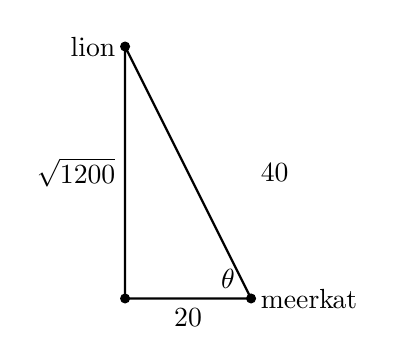
\begin{tikzpicture}[scale=0.4]
     \draw[thick](0,0) -- (0,-8) -- (4,-8) -- (0,0);
     \node[left] at (0,0){lion};
     \node[left] at (0,-8){};
     \node[right] at (4,-8){meerkat};
      \node[anchor=south east] at (3.8,-8){$\theta$};
     \draw[fill] (0,0) circle [radius=4pt];
     \draw[fill] (0,-8) circle [radius=4pt];
     \draw[fill] (4,-8) circle [radius=4pt];
     \node[left] at (0,-4){$\sqrt{1200}$};
     \node[below] at (2,-8){$20$};
     \node[right] at (4,-4){$40$};
    
     \end{tikzpicture}
     \end{center}
    \end{solution}
    \vfill\vfill
    \newpage
\item Using your work on the previous page, answer the following questions:
\begin{enumerate}
    \item 
    \begin{workshop}
    There is more than one possible equation that relates $y$ and $\theta$, so students might need some prompting to realize which equation is most efficient to use before differentiation.
    \end{workshop}
    At the moment when the lion is $40$ feet from the meerkat and getting closer, how fast is the meerkat's head turning (in radians per second)?
    
    \begin{solution}
        Let's relate the variables $\theta$ and $y$ because we want to know $\frac{d\theta}{dt}$ and we already know $\frac{dy}{dt}$. At this stage, we can relate $\theta$ and $y$ with either sine or tangent. If we used sine, the equation that relates our variables would contain an additional variable $z$ that, when differentiated with respect to time, would generate the quantity $\frac{dz}{dt}$, which we also don't yet know. (However, if we did know $\frac{dz}{dt}$, which we would after solving the next part of this question, this method would work just fine.) So, let's use tangent:
    \begin{align*}
            \tan \theta &= \frac{y}{20} \\
            20 \tan \theta &= y
    \end{align*}
    Now, let's differentiate with respect to time and plug in information we know from our snapshot and the problem statement:
    \begin{align*}
            \frac{d}{dt}(20 \tan \theta) &= \frac{d}{dt}(y) \\
            20\sec^2 \theta \cdot \frac{d\theta}{dt}&= \frac{dy}{dt} \\
            \frac{d\theta}{dt}&=\frac{1}{20}\cos^2 \theta \cdot \frac{dy}{dt} \\
            \frac{d\theta}{dt}&=\frac{1}{20}\left(\frac{20}{40}\right)^2 (-60) \\
            &=-\frac{3}{4}\text{ radians per second}
    \end{align*}
    \end{solution}
    \vfill\vfill
    \item
    \begin{workshop}
   This is a problem students could have solved before our trigonometry unit by using the Pythagorean Theorem. 
    \end{workshop}
    
    At the moment when the lion is $40$ feet from the meerkat and getting closer, at what rate is the distance between the lion and the meerkat shrinking?
    
    \begin{solution}
        Let's relate the variables $y$ and $z$ since we are looking for $\frac{dz}{dt}$ when $z=40$ and we know $\frac{dy}{dt}$.
    \begin{align*}
        20^2+y^2=z^2
    \end{align*}
    Now, let's differentiate with respect to time and plug in information we know in the moment when $z=40$ to solve for $\frac{dz}{dt}$.
    \begin{align*}
        \frac{d}{dt}(20^2+y^2)&=\frac{d}{dt}(z^2) \\
        2y\frac{dy}{dt}&=2z\frac{dz}{dt} \\
        y\frac{dy}{dt}&=z\frac{dz}{dt} \\
        (\sqrt{1200})(-60)&=40\frac{dz}{dt} \\
        \frac{dz}{dt}&=\frac{(\sqrt{1200})(-60)}{40}\\
        &=-30\sqrt{3}\text{ feet per second}
    \end{align*}
    \end{solution}
    \vfill


\end{enumerate}
\end{enumerate}
\newpage
\begin{workshop}
    This question (\#6a-c) is an exam-type problem. Even if most students don't get to it, feel free to preview it with students and encourage them to complete it on their own time.
\end{workshop}
    \item In this question we will explore the properties of $f(x)=e^x\sin x$.
    \begin{enumerate}
    \item Find all $x$- intercepts of $y=f(x)$ on $[-2\pi, 2\pi]$. 


    \begin{solution}
    Here we solve the equation $e^x\sin x=0$ on the interval $[-2\pi, 2\pi]$. Since $e^x$ is never equal to $0$, we solve $\sin x =0$ on $[-2\pi, 2\pi]$. Thus, \fbox{$x=-2\pi, -\pi, 0, \pi, 2\pi$}.
    \end{solution}
    \vfill
    \item Where is $f(x)$ increasing on $[0, 2\pi]$? Where is it decreasing on $[0, 2\pi]$?
    
    \begin{solution}
        Let's find $f'(x)$ and set it equal to 0 to find the critical points on the interval $[0, 2\pi]$.
        \begin{align*}
            f'(x)&=e^x\sin x+e^x\cos x \\
            0&=e^x\sin x+e^x\cos x \\
            0&=e^x(\sin x+\cos x) \\
        \end{align*}
        Since $e^x$ is never equal to 0,
        \begin{align*}
            0&=\sin x+\cos x \\
            -\sin x&=\cos x \\
            -\tan x &= 1 \\
            x &= \frac{3\pi}{4}, \frac{7\pi}{4}
        \end{align*}
        Now, let's test $f'$ at points that fall between each end point and critical point for their sign:
        \begin{align*}
            f'\left(\frac{\pi}{2}\right)&=e^{(\pi/2)}\left[\sin\left(\frac{\pi}{2}\right)+\cos\left(\frac{\pi}{2}\right)\right]=e^{(\pi/2)}>0\\
            f'(\pi)&=e^{\pi}(\sin\pi +\cos\pi)=e^{\pi}(-1)<0\\
            f'\left(\frac{11\pi}{6}\right)&=e^{(11\pi/6)}\left[\sin\left(\frac{11\pi}{6}\right)+\cos\left(\frac{11\pi}{6}\right)\right]=e^{(11\pi/6)}\left(\frac{\sqrt{3}}{2}-\frac{1}{2}\right)>0\\
        \end{align*}
        Thus, $f(x)$ increases on $[0, \frac{3\pi}{4}]$ and $[\frac{7\pi}{4}, 2\pi]$ and decreases on $[\frac{3\pi}{4}, \frac{7\pi}{4}]$. 
    \end{solution}
    \vfill\vfill\vfill
   

       
    \item Based on your answers to parts (a) and (b), which one of the following is the best sketch of $y=f(x)$? Please circle your choice.
    \solonly{\textcolor{red}{Choice B is the only graph that has equally spaced $x$-intercepts and is increasing and decreasing on the intervals we found.}}

% \begin{center}
%     \begin{figure}[h]
%         \centering
%         \includegraphics[scale=0.5]{Graphs.png}
%         \end{figure}
% \end{center}



\begin{center}
\begin{tikzpicture}
    \begin{groupplot}[
        group style = {group size=3 by 2},
        grid = none,
        xtick=\empty,
        ytick=\empty,
        width = 2.3in,
        xmin=-8, xmax=8, ymin=-3, ymax=3,
        restrict y to domain=-100:100]

    \nextgroupplot[title=(A)]
    \addplot[draw=none] coordinates {(0,0)};
    \addplot[domain = -8:8, color = black]{sin(deg(x^2/2)};

    \nextgroupplot[title=(B)]
    \addplot[draw=none] coordinates {(0,0)};
    \addplot[domain = -8:8, color = black]{0.8*e^(0.2*x) * sin(deg( x)};

    \nextgroupplot[title=(C)]
    \addplot[draw=none] coordinates {(0,0)};
    \addplot[domain = -8:8, color = black]{-0.8*e^(-0.2*x)*sin(deg(x)};
    \end{groupplot}
\end{tikzpicture}
\end{center}
\end{enumerate}

\newpage
\begin{workshop}
    Envelope functions are exploratory material that will not be assessed in Math Mb, although they can be helpful when sketching trig functions or in later courses like Math 1b that include content about bounding.
\end{workshop}
\item (\textit{Exploratory}) Another method to have chosen an answer to \#6c is to identify bounds, or ``envelopes", that smoothly outline the extremes in amplitude of $f(x)$. Below, we will investigate how the minima and maxima of the function's oscillations change, and how we describe that change.
\begin{center}
\begin{tikzpicture}
    \begin{groupplot}[
        group style = {group size=1 by 1},
        grid = none,
        xtick=\empty,
        ytick=\empty,
        width = 3in,
        xmin=-8, xmax=8, ymin=-3, ymax=3,
        restrict y to domain=-100:100]

   
   

    \nextgroupplot
    \addplot[draw=none] coordinates {(0,0)};
    \addplot[domain = -8:8, color = black]{0.8*e^(0.2*x) * sin(deg( x)};
    \addplot[dashed][domain = -8:8, color = black]{0.8*e^(0.2*x) };
    \addplot[dashed][domain = -8:8, color = black]{-0.8*e^(0.2*x) };

    
    \end{groupplot}
\end{tikzpicture}
\end{center}
\begin{enumerate}
    \item 
    The graphs of $f(x)=e^x\sin x$ and its \textit{envelope} functions, $y=e^x$ and $y=-e^x$, are shown above. Label each of the three curves above with their respective formulas. 
    
    \begin{solution}
        The oscillating curve in black is $f(x)=e^x\sin x$. The dotted curve above it is $y=e^x$, and the dotted curve below it is $y=-e^x$. 
    \end{solution}
    \vfill
    \item What do you notice about the relative position of $f(x)=e^x\sin x$ and its envelope functions?
    
    \begin{solution}
        The graph of $f(x)=e^x\sin x$ oscillates between and periodically intersects the envelopes $y=e^x$ and $y=-e^x$. In other words, the plots of $y=e^x$ and $y=-e^x$ provide bounds that smoothly outline the varying minima and maxima of $f(x)$. 
    \end{solution}
   \vfill\vfill\vfill\vfill
    
    \item Using your knowledge of the range of $\sin x$, explain why the following inequality is true.
     \[
        {-e^x} 
        \hspace{6pt} \leq \hspace{6pt}
       e^x \sin x
        \hspace{6pt} \leq \hspace{6pt}
        {e^x}
\]

    \begin{solution}
    The range of $\sin x$ is $[-1,1]$, which is to say that $-1\leq \sin x\leq 1$. Multiplying each term in this inequality by $e^x$ yields $-e^x\leq e^x\sin x\leq e^x$. For any $x$, since $\sin x$ must lie at or in between $-1$ and $1$, $e^x\sin x$ must also lie at or in between $-e^x$ and $e^x$.
    \end{solution}
    
    \vfill \vfill \vfill\vfill
 

\begin{framed}
    Envelope functions provide ``tight" bounds -- or the  ``highest floor" and ``lowest ceiling" -- that smoothly outline the extremes in amplitude of an oscillating curve. Identifying envelope functions is a helpful curve sketching tool for oscillations whose amplitudes or balance lines are not constant.
\end{framed}


\newpage


\item Match the following functions with their graphs (not to scale) below. (It might be helpful to directly draw in the two envelope functions that outline each oscillating curve graphed below!)

\begin{enumerate}
    

\begin{multicols}{3}
    \item \fitb{0.4in}{
      \solonly\textcolor{red}{C}
      } $y=x\sin x$
    \vspace{0.5cm}
    \item \fitb{0.4in}{
      \solonly\textcolor{red}{D}
      } $y=x^2\sin x$
    \vspace{0.5cm}
    \item \fitb{0.4in}{
      \solonly\textcolor{red}{A}
      } $y=\dfrac{\sin x}{x}$
    \vspace{0.5cm}
    \item \fitb{0.4in}{
      \solonly\textcolor{red}{H}
      } $y=e^{-x}\sin x$
    \vspace{0.5cm}
    \item \fitb{0.4in}{
      \solonly\textcolor{red}{G}
      } $y=\sin x + x$
    \vspace{0.5cm}
    \item \fitb{0.4in}{
      \solonly\textcolor{red}{F}
      } $y= \sin(20x)\sin x$
    \vspace{0.5cm}
    
   
    
    \item \fitb{0.4in}{
      \solonly\textcolor{red}{E}
      } $y=e^{x}\sin x$
    \vspace{0.5cm}
    \item \fitb{0.4in}{
      \solonly\textcolor{red}{B}
      } $y=\sin x - x$
    \vspace{0.5cm}
    \item \fitb{0.4in}{
      \solonly\textcolor{red}{I}
      } $y= (\ln x)\sin x$
    \vspace{0.5cm}
    
    
\end{multicols}
\end{enumerate}
% \begin{center}
%     \begin{figure}[h]
%         \centering
%         \includegraphics[scale=0.5]{Graphs.png}
%         \end{figure}
% \end{center}

\vspace{0.5cm}

\begin{center}
\begin{tikzpicture}
    \begin{groupplot}[
        group style = {group size=3 by 3},
        grid = none,
        xtick=\empty,
        ytick=\empty,
        width = 2.3in,
        xmin=-70, xmax=70, ymin=-70, ymax=70,
        restrict y to domain=-100:100,
        samples=300]
        
    \nextgroupplot[title=(A)]
    \addplot[draw=none] coordinates {(0,0)};
    \addplot[domain = -70:70, color = black]{(50/x) * sin(deg(x)};
   \solonly{
    \addplot[domain = -70:70, color = red]{(50/x)};
    \addplot[domain = -70:70, color = red]{(-50/x)};
   
    }
    
    \nextgroupplot[title=(B)]
    \addplot[draw=none] coordinates {(0,0)};
    \addplot[domain = -70:70, color = black]{10*sin(deg(x))-x};
    \solonly{
    \addplot[domain = -70:70, color = red]{10-x};
    \addplot[domain = -70:70, color = red]{-10-x};
    }
    
    
    \nextgroupplot[title=(C)]
    \addplot[draw=none] coordinates {(0,0)};
    \addplot[domain = -70:70, color = black]{x * sin(deg(x)};
\solonly{
    \addplot[domain = -70:70, color = red]{(x)};
    \addplot[domain = -70:70, color = red]{(-x)};
   
    }

    \nextgroupplot[title=(D)]
    \addplot[draw=none] coordinates {(0,0)};
    \addplot[domain = -70:70, color = black]{(0.03 * x^2) * sin(deg(x))};
\solonly{
    \addplot[domain = -70:70, color = red]{(0.03 * x^2};
    \addplot[domain = -70:70, color = red]{(-0.03 * x^2)};
   
    }
     \nextgroupplot[title=(E)]
    \addplot[draw=none] coordinates {(0,0)};
    \addplot[domain = -70:70, color = black]{e^(0.07*x)*sin(deg(x)};
    \solonly{
    \addplot[domain = -70:70, color = red]{e^(0.07*x)};
    \addplot[domain = -70:70, color = red]{-e^(0.07*x)};
   
    }
    
    \nextgroupplot[title=(F)]
    \addplot[draw=none] coordinates {(0,0)};
    \addplot[domain = -70:70, color = black]{40*sin(deg(0.09*x))*sin(deg(1.3*x)};
    \solonly{
    \addplot[domain = -70:70, color = red]{40*sin(deg(0.09*x))};
    \addplot[domain = -70:70, color = red]{-40*sin(deg(0.09*x))};
   
    }

    \nextgroupplot[title=(G)]
    \addplot[draw=none] coordinates {(0,0)};
    \addplot[domain = -70:70, color = black]{10*sin(deg(x))+x};
    \solonly{
    \addplot[domain = -70:70, color = red]{10+x};
    \addplot[domain = -70:70, color = red]{x-10};
   
    }

    \nextgroupplot[title=(H)]
    \addplot[draw=none] coordinates {(0,0)};
    \addplot[domain = -70:70, color = black]{e^(-0.07*x)*sin(deg(x)};
\solonly{
    \addplot[domain = -70:70, color = red]{e^(-0.07*x)};
    \addplot[domain = -70:70, color = red]{-e^(-0.07*x)};
   
    }
    
    \nextgroupplot[title=(I)]
    \addplot[draw=none] coordinates {(0,0)};
    \addplot[domain = -70:70, color = black]{10*ln(x)*sin(deg(x))};
\solonly{
    \addplot[domain = -70:70, color = red]{10*ln(x)};
    \addplot[domain = -70:70, color = red]{-10*ln(x)};
   
    }
    
    
    \end{groupplot}
\end{tikzpicture}
\end{center}


\end{enumerate}
\end{enumerate}
\end{document}
